\setchapterpreamble[u]{\margintoc}
\chapter{Methodology}
\labch{method}

%---------------------------------------------------------------
% overview of chapter 
In this chapter, we describe the basic numerical methodology behind our models 
concerning the dynamics of immiscible liquid-gas interfacial flows, at the incompressible and isothermal limits. 
These implementations are developed on the platforms 'PARIS Simulator' \cite{paris} and 
'Basilisk' \cite{basilisk}, with considerable overlap between the two platforms in terms 
of the treatment of the interface capturing schemes, transport of conserved quantities and surface tension models.
\sidenote{The principle difference between 'PARIS Simulator' and 'Basilisk' is the ability to resolve the conservation
laws on dynamically adaptive meshes in the case of 'Basilisk', whereas 'PARIS Simulator' only deals with regular Cartesian meshes.}
The numerical implementations are based on finite volume discretizations on uniform or dynamically refined Cartesian grids , utilizing
state of the art methods in interfacial reconstruction coupled with geometric
transport of the corresponding fluxes, curvature computation and surface tension modeling. For more detailed
descriptions of the general capabilities of 'PARIS Simulator’ and 'Basilisk', we refer the reader to the previously cited references. 


\section{Governing Equations}

We use the one-fluid formulation for our system of governing equations, thus solving 
the incompressible Navier-Stokes equations throughout the whole domain including regions 
of variable density and viscosity, which itself depend on the explicit 
location of the interface separating the two fluids.
In the absence of mass tranfer, the velocity field is continuous across
the interface at the incompressible limit, with the interface evolving according to the local velocity vector.  

\subsection*{Conservative Formulation}

Generally, we have a choice regarding how to model the convective operator
of the incompressible Navier-Stokes equations. There is a well established corpus of 
numerical methods tailored specifically to deal with non-conservative 
\sidenote{also referred to as the strong form, necessitating certain orders of smoothness of the primitive variable} form of the convective 
operator that appear in transport equations of mass and momentum 
\sidenote{These methods are descendants of the class of numerical schemes used to solve hyperbolic partial differential equations.}
, which perform quite well in the context of single phase flows.
However, in interfacial flows we often deal with discontinuities that arise as a consequence
of the contrast in material properties between the two fluids. Therefore, even though the velocity field
remains continuous throughout the domain, the otherwise smooth density (mass) and momentum fields 
contain sharp jumps (discontinuities) localized at the interfacial position.     
Therefore, we choose to formulate our governing equations in a conservative form i.e involving divergence of fluxes instead of gradients of the primitive variables when it comes to the convective operator. More detailed discussions and analyses about the comparative advantages of the conservative formulation in the context of flows involving large density-ratios is the focus of the subsequent chapters. Thus, the equations are as follows :  



% in incompressible flows, the velocity field is continuous in the absence of mass transfer across the interface 

\begin{align} 
	\frac{\partial \rho}{\partial t} + \nabla\cdot \left(\rho\boldsymbol{u}\right) &= 0 \label{mass} \\
	\frac{\partial}{\partial t} \left(\rho\boldsymbol{u}\right) + \nabla\left(\rho\boldsymbol{u}\otimes\boldsymbol{u}\right)  &= -\nabla p + \nabla \cdot \left(2 \mu \boldsymbol{D}\right) + \sigma \kappa \delta_{s}\boldsymbol{n} + \rho \boldsymbol{g}
\label{nseqn}
\end{align}


with $\rho$ and $\mu$ being the density and dynamical viscosity respectively, and therefore are the physical quantities which are discontinuous across the interface. The volumetric sources are modeled by the acceleration $g$, and the deformation rate tensor $\boldsymbol{D}$ used to model the viscous stresses is defined as:  

\begin{align}
	\boldsymbol{D} = \frac{1}{2}\left[\nabla \boldsymbol{u} + \left(\nabla \boldsymbol{u}\right)^{T}\right]  
\end{align}


The term $\sigma \kappa \delta_{s}\boldsymbol{n}$ models the surface tension forces in the 
framework of the continuum surface-force (CSF) method. The normal vector to the interface 
is $\boldsymbol{n}$, with $\sigma$ being the coefficient of surface tension and $\kappa$ the 
local interfacial curvature. The operator $\delta_{s}$ is the Dirac delta function, 
the numerical approximation of which allows us to map the singular surface force distribution
along the interface onto their volumetric equivalents for our Cartesian control volumes. 
At the incompressible limit, the advection of mass given by equation \ref{mass} can be 
treated as equivalent to that of the advection of volume.


\subsection*{Material Properties}
Within the framework of interface capturing schemes, the 
temporal evolution of the interface separating the two fluids
can be modeled by the following advection equation : 

\begin{align} 
	\frac{\partial \chi}{\partial t} + \boldsymbol{u}\nabla\chi = 0 	
\label{chi}
\end{align}

where $\chi$ is the phase-characteristic function, that has different values 
in each phase \sidenote{Generally, $\chi$ is assigned values of $0$ in one phase and $1$ in the other. } . Mathematically, the function $\chi$
is equivalent to a Heaviside function in space and time. 
At the macroscopic length scales under consideration, the interface evolution
as described by equation \ref{chi} is modeled as having infinitesimal thickness
under the continuum hypothesis. The coupling of the interfacial evolution with
the equations of fluid motion as described in \ref{mass} and \ref{nseqn} is provided by :  

\begin{align}
	\rho &= \rho_{1}\chi + \left(1 - \chi\right)\rho_{2} \label {rho_chi} \\ 
	\mu  &= \mu_{1}\chi  + \left(1 - \chi\right)\mu_{2}  
  \label{mu_chi}
\end{align}

where $\rho_{1}$, $\rho_{2}$ are the densities of fluids 1 and 2 respectively, 
likewise for viscosities $\mu_{1}$ and $\mu_{2}$. Under certain circumstances, 
it is beneficial to opt for a weighted harmonic mean description of the 
variable dynamic viscosity, instead of the weighted arithmetic mean as in equation \ref{mu_chi}. 


The two main (and the most popular)
approaches in the context of interface capturing schemes are the 
are the volume-of-fluid (VOF) method first developed by Hirt and Nichols \cite{hirt1981volume}, 
and the level set class of methods pioneered by Osher and Sethian \cite{osher1988fronts}.
The principal difference between the two approaches lies in the manner in which
the Heaviside function $\chi$ is modeled in the discrete sense, 
either as a smooth differentiable field in
the case of level sets, or as a sharp discontinuous field in the volume-of-fluid (VOF) context.  
Each class of methods has its own set of merits (and demerits) relative to each other. 
Generally speaking, volume-of-fluid based methods display superior mass conservation
\sidenote{VOF based methods implicitly track the evolution of the discontinuous density field, 
which is not the case in level set based methods. }
whereas in terms of interface curvature computation, level set based methods hold an advantage
\sidenote{The differentiable nature of the level set function lends itself
to straightforward curvature computation routines. } . 
A detailed exposition into the different classes of interfacial transport
methods can be found in the seminal monograph by Tryggvason, Scardovelli and Zaleski \cite{zaleskibook}

%---------------------------------------------------------------

\section{Interfacial Transport : VOF}
Our numerical studies are based on the Volume-of-Fluid methodology. 
We refer to the discontinuous approximation to the Heaviside function
\sidenote{A comprehensive discussion about the different types of approximations
to the interface Heaviside function can be found in Popinet \cite{popinet2018numerical}}
$\chi$ as the volume fraction field or colour function interchageably, which 
is defined below in the context of finite volume discretization : 

\begin{align} 
	C_{ijk}\left(t\right) = \frac{1}{\Delta V} \displaystyle\int_{\Delta V} \chi(\boldsymbol{x},t) \,d\boldsymbol x 
\end{align}

where $C$ is the colour function with its values lying between $0$ and $1$, 
with $i$,$j$ and $k$ being the indices to the corresponding discretized control volume of volume $\Delta V$.  
There are two steps involved in the VOF method, the reconstruction of the interface and its 
subsequent propagation (advection). We present a brief overview of the two steps in the following sections,
as going into detailed descriptions of the reconstruction and propagation procedures are 
not the focus of the present body of work \sidenote{In-depth explanations into these numerical 
techniques can be found in \cite{zaleskibook, zaleskiannual,vof_1,vof_2}.}.  


\subsection*{PLIC representation}
We employ means of geometric reconstructions to explicitly define the 
interface location using the discrete colour function information. 
The interface is represented by disjointed line segments under 
the PLIC (piecewise linear interface construction)
framework as illustrated in figure \ref{vof_plic}, with the images reproduced 
from the the review by Scardovelli and Zaleski \sidecite{zaleskiannual}. 
Such reconstructions involve the determination of interface normals 
using the Mixed Youngs Centered method, the detailed description 
of which can be found in \cite{zaleskibook}. 

\begin{figure}[!h]
\begin{center}
\begin{tabular}{cc}
\hspace*{-1.0cm}
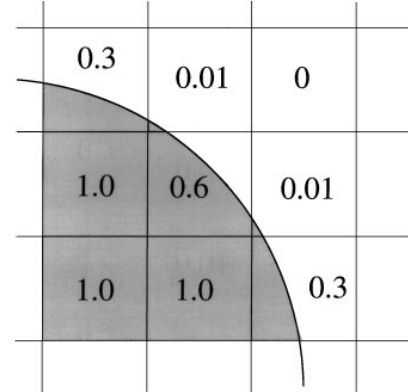
\includegraphics[width=0.5\textwidth]{plots/methodology/vof_basic.png} &
\hspace{-0.2cm}%
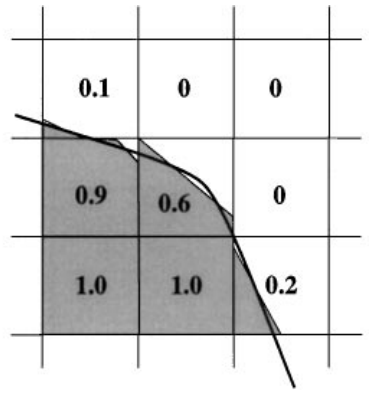
\includegraphics[width=0.473\textwidth]{plots/methodology/vof_plic.png} \\ 
\hspace{-0.2cm}%
(a) & (b) \\
\end{tabular}
\end{center}
\caption{ Exlicit definition of the interface location using the volume-of-fluid approach. 
These images are reproduced with permission from Scardovelli and Zaleski \cite{zaleskiannual}.
(a) The exact discrete representation of a circular arc on a regular Cartesian grid using the colour function field (volume fraction).
(b) The piecewise linear (PLIC) approximation to the smooth circular arc shown in (a), which entails second-order spatial accuracy.   
}
\label{vof_plic}
\end{figure}

\subsection*{Flux Computation}
Once the geometric PLIC reconstructions have been carried out, 
the interface segments are advected using the the velocity field. 
This entails computation of fluxes of the colour function, which 
can be computed via algebraic transport schemes (generally less accurate), 
or by using geometric reconstructions in either Eulerian, Lagrangian or hybrid frameworks.
In the context of our numerical platforms (`PARIS' and `Basilisk'), 
state-of-the-art \sidenote{The reader can refer to 
\cite{paris,basilisk} for further details}  
geometrical flux reconstruction procedues are utilised. 
The temporal integration of the fluxes could be carried out either as a 
series of one dimensional propagations along each of the spatial directions, 
termed as direction-split, or carried out in one single sweep, 
termed as multidimensional or unsplit.

Direction-split methods are more intuitive and easier to develop (extension to 
3D in particular), but suffer from lack of conservation (to the order of 
machine precision) when it comes to 3D \sidenote{
A detailed exposition of this problem along with a noteworthy solution  
can be found in the work by Weymouth and Yue \cite{wy}}. 
Multidimensional (unsplit) methods have an advantage in that respect due to the 
fact that they are conservative by nature of their design, but are inherently 
more complicated to develop and implement, with no straightforward extension from 2D to 3D.    
For a more detailed and nuanced evaluation of the comparitive advantages of 
interfacial transport methods, we refer the reader to the recent review by 
Mirjalili et al. \cite{mirjalili2017interface} on the given subject.     
The propagation of the interface can be described by the evolution of
the colour function (volume fraction field) as - 

\begin{align} 
	\frac{\partial C}{\partial t} + \boldsymbol{u} \cdot \nabla C = 0  	
\label{cvof_non}
\end{align}

We can express the same in the conservative form as - 

\begin{align} 
	\frac{\partial C}{\partial t} + \nabla \cdot \left(C \boldsymbol{u}\right) = C \left(\nabla \cdot \boldsymbol{u}\right) 	
\label{cvof_con}
\end{align}

As one can observe, the ``compression'' term on the right hand side of equation 
\ref{cvof_con} equals to zero in the context of incompressible flows without mass 
transfer, but it is important to keep this term in our numerical formulation within 
the direction-split framework. Discretization of the above equation results in :

\begin{align}
	C_{i,j,k}^{n,d+1} = C_{i,j,k}^{n,d} - F_{+}^{n,d}\left(C \right) - F_{-}^{n,d}\left(C \right) + \overline{C}_{i,j,k}^{n,d}\left(\frac{\Delta u}{\Delta x}\right)^{n,d}_{i,j,k}  
  \label{cvof_discrete}
\end{align}

The above equation represents an advection substep, the superscripts $n$ and $d$ refer to the timestep and 
direction of integration respectively. The notation $d=0$ refers to the field 
at the $n^{th}$ timestep, before any integration is performed along any direction. 
The fluxes $F_{\pm}^{n,d}(C)$ in equation \ref{cvof_discrete} are derived through geometrical reconstructions. 
After each substep, the interface is reconstructed once again with the updated 
volume fraction field in order to compute the fluxes for the next advection substep.  
Finally, the volume fraction field for the next timestep is given by -

\begin{align}
	 C^{n+1}_{i,j,k} = C^{n,3}_{i,j,k}  
\end{align}

The interpretation and numerical approximation of the prefactor $\overline{C}_{i,j,k}^{n,d}$ 
to the directional divergence, as well as the fluxes $F_{\pm}^{n,d}(C)$, depend 
on the exact nature of the geometrical advection scheme in question, 
which in our context is either CIAM (Lagrangian explicit) or Weymouth-Yue (Eulerian implicit) 
\sidenote{The classification of Lagrangian explicit and Eulerian implicit 
are in accordance with the paper by Aulisa et al. \cite{aulisa2003}}.
A brief outline of these two methods is presented in the subsequent sections.   

\paragraph{Lagrangian Explicit} 
This scheme was originally described in the work of Li \cite{li95}, `CIAM' being an 
abbreviation for the French title `\textit{Calcul d'interface affine par morceaux}', 
which can be thought of as a straightforward Lagrangian transport of the interface Heaviside function. 
After the interface segments are reconstructed from the discrete colour function 
at the start of the time-step, the interfacial points are transported by the component of the 
velocity field \sidenote{The temporal integration of the position
is carried out using a first-order explicit estimate in time, 
along with a linear interpolation of the component of the velocity field.}
corresponding to the direction of transport. A geometrical interpretation of the scheme
is illustrated in figure \ref{ciam}, reproduced from the seminal work of Gueyffier et al. \cite{gueyffier}. 
\begin{figure}[!h]
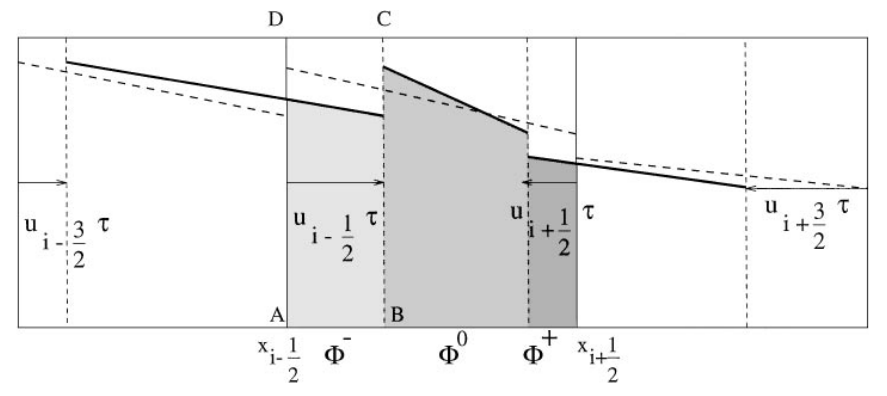
\includegraphics[width=1.0\textwidth]{plots/methodology/ciam.png} 
\caption{
Lagrangian transport of the interface segments using the CIAM scheme, the image
is reproduced with permission from Gueyffier et al. \cite{gueyffier}. 
A 2D schemetic of the geometric calculation of the fluxes of the volume 
fraction field is shown, for the advection substep along the horizontal direction.
The central cell ($i,j,k$) undergoes a net compression during this substep.
The fluxes $\Phi^{-}$ , $\Phi^{0}$ and $\Phi^{+}$ are the volumes under the 
advected interface segments advected by the interpolated velocity field,
intersected by the $(i,j,k)$ cell boundaries. 
}
\label{ciam}
\end{figure}

As one can infer from the geometrical representation in figure \ref{ciam}, 
the fluxes $F_{\pm}^{n,d}(C)$ correspond to the volumes $\Phi^{-}$ and $\Phi^{+}$. 
Thus, the updated field $C_{i,j,k}^{n,d+1}$ is the sum of the 
three contributions $\Phi^{-}$ , $\Phi^{0}$ and $\Phi^{+}$. 
We can rewrite equation \ref{cvof_discrete} specifically for the CIAM scheme as -  

\begin{align}
C_{i,j,k}^{n,d+1} =  C_{i,j,k}^{n,d}\left[1 + \left(\frac{\Delta u}{\Delta x}\right)^{n,d}_{i,j,k} \right] - F_{+}^{n,d}\left(C \right) - F_{-}^{n,d}\left(C \right)   
\label{ciam_discrete}
\end{align}

where the compression coefficient $\overline{C}_{i,j,k}^{n,d}$ is simply equal 
to the value of the colour function $C_{i,j,k}^{n,d}$ at the start of the 
corresponding advection substep. Although the flux terms cancel upon integration 
throughout the whole domain, one can clearly see that the compression terms do 
not sum up to zero due to the changing prefactor in front of the directional divergences. 
This precise issue brings us to the next advection scheme.      

\paragraph{Eulerian Implicit}
This advection scheme was developed by Weymouth and Yue \cite{wy} in order to 
specifically tackle the problem of discrete conservation when it comes to direction-split 
geometrical advection schemes \sidenote{By `discrete conservation' we mean that the sum of 
the directional divergences sum upto zero, to the accuracy of machine precision.}. 
The scheme fundamentally employs a forward Eulerian method in order to carry out temporal 
integration of the fluxes, with the fluxes themselves computed as the quantity of the substance 
entering or exiting a given control volume through its fixed surfaces. 

\begin{align}
	\overline{C}_{i,j,k}^{n,d} &= 0 \quad \text{if} \quad C_{i,j,k}^{n,0} < 0.5 \\
	\overline{C}_{i,j,k}^{n,d} &= 1 \quad \text{if} \quad C_{i,j,k}^{n,0} \geq 0.5 
\end{align}

%---------------------------------------------------------------

\section{Time Marching}

\subsection*{Spatio-Temporal Discretization}
\blindtext

\subsection*{Pressure-Poisson Projection}
\blindtext

\section{Source Terms}

\subsection*{Surface Tension}


\subsection*{Viscous Diffusion}

\blindtext
